%=====================================================================
%  SEGUNDA ENTREGA - PROCESAMIENTO DIGITAL DE IMAGENES
%  Formato IEEE (IEEEtran, conference)
%
%  Contenido: Introduccion, Planteamiento, Justificacion, Estado del
%  arte, METODOLOGIA y Resultados parciales.
%=====================================================================

\documentclass[conference]{IEEEtran}

\usepackage[utf8]{inputenc}
\usepackage[T1]{fontenc}
% Si su distribucion tiene spanish.ldf (Overleaf, TeX Live completo),
% puede usar:  \usepackage[spanish,es-noquoting]{babel}
\usepackage[spanish,provide=*]{babel}
\usepackage{amsmath,amssymb,amsfonts}
\usepackage{graphicx}
\usepackage{booktabs}
\usepackage{array}
\usepackage{url}
\usepackage{textcomp}
\usepackage{algorithmic}

\addto\captionsspanish{%
  \renewcommand{\tablename}{Tabla}%
  \renewcommand{\figurename}{Fig.}%
}

\begin{document}

\title{Detección de reproducciones impresas de billetes colombianos\\
mediante análisis de textura y espectro de impresión,\\
con interfaz accesible para personas con discapacidad visual}

\author{
\IEEEauthorblockN{Juan Castaño}
\IEEEauthorblockA{Cód. 1202720\\
Ingeniería Multimedia\\
Universidad Militar Nueva Granada}
\and
\IEEEauthorblockN{Nicolás Moreno}
\IEEEauthorblockA{Cód. 1202437\\
Ingeniería Multimedia\\
Universidad Militar Nueva Granada}
\and
\IEEEauthorblockN{Andrés Navia}
\IEEEauthorblockA{Cód. 1202517\\
Ingeniería Multimedia\\
Universidad Militar Nueva Granada}
}

\maketitle

%=====================================================================
\renewcommand{\abstractname}{Abstract}
\begin{abstract}
Cash remains the dominant payment method across large segments of the
Colombian economy, and receiving a non-genuine banknote is an
unrecoverable loss. The risk falls disproportionately on people who
cannot perform the conventional visual inspection. Existing electronic
banknote readers designed for this population identify denomination but
do not assess authenticity.

This document reports the methodology and the partial results of a
digital image processing system that recognizes denomination and
discriminates between genuine banknotes and printed reproductions.
Every operation is implemented from its mathematical definition over
numerical arrays, without computer vision libraries: object region
extraction by two-pass connected component labelling, boundary
following by Moore's algorithm, minimum-area rectangle fitting by
rotating calipers, and perspective rectification by explicitly solving
the eight-by-eight system posed by the direct linear transformation,
followed by inverse mapping with bilinear interpolation.

Segmentation does not rely on a single cue. Four complementary saliency
maps are generated and, over a grid of morphological scales, the region
whose minimum-area rectangle best matches the known aspect ratio of a
banknote is selected. This replaces the need to guess in advance which
cue works under which illumination.

The central experimental contribution is a paired design. Earlier
comparisons contrasted photographs taken at different times and with
different cameras, so any measured difference could stem either from
printing or from capture conditions. Two discard tests failed to
explain the observed separation: degrading the genuine images through
the same compression chain did not reproduce it, and edge sharpness
measurements showed the reproductions were in fact better focused. A
genuine and a didactic banknote were then photographed within the same
frame, which controls capture conditions by construction. Across two
denominations, the reproductions show between twenty-five and one
hundred times less Laplacian energy while their physical edge is
sharper, establishing that the microtexture difference is a property of
the printing and not of the photograph.
\end{abstract}

\renewcommand{\abstractname}{Resumen}
\begin{abstract}
Este documento reporta la metodología y los resultados parciales de un
sistema de procesamiento digital de imágenes que reconoce la
denominación de billetes colombianos y discrimina entre ejemplares
auténticos y reproducciones impresas.

Todas las operaciones se implementan a partir de su definición
matemática sobre arreglos numéricos, sin recurrir a librerías de visión
artificial: la extracción de la región del objeto por etiquetado de
componentes conexas de dos pasadas, el seguimiento de frontera por el
algoritmo de Moore, el ajuste del rectángulo de área mínima por
calibradores rotantes, y la rectificación proyectiva resolviendo
explícitamente el sistema de ocho ecuaciones de la transformación
lineal directa, seguido de un remapeo inverso con interpolación
bilineal.

La segmentación no descansa en una sola evidencia. Se generan cuatro
mapas de saliencia complementarios y, sobre una rejilla de escalas
morfológicas, se selecciona la región cuyo rectángulo de área mínima
mejor se ajusta a la relación de aspecto conocida de un billete. Esto
sustituye la necesidad de acertar de antemano qué evidencia funciona
bajo cada iluminación.

La contribución experimental central es un diseño pareado. Las
comparaciones previas contrastaban fotografías tomadas en momentos y
con cámaras distintas, de modo que cualquier diferencia podía provenir
de la impresión o de la condición de captura. Dos pruebas de descarte
no lograron explicar la separación observada: degradar las imágenes
auténticas con la misma cadena de compresión no la reprodujo, y la
medición de agudeza de borde mostró que las reproducciones estaban
incluso mejor enfocadas. Se fotografió entonces un billete auténtico y
uno didáctico dentro del mismo encuadre, lo que controla la condición
de captura por construcción. En dos denominaciones, las reproducciones
presentan entre veinticinco y cien veces menos energía en el laplaciano
mientras su borde físico es más agudo, lo que establece que la
diferencia de microtextura es una propiedad de la impresión y no de la
fotografía.
\end{abstract}

\begin{IEEEkeywords}
Procesamiento digital de imágenes, segmentación, morfología matemática,
homografía, transformada de Fourier, análisis de textura, LBP, GLCM,
accesibilidad, discapacidad visual.
\end{IEEEkeywords}

%=====================================================================
\section{Introducción}

El efectivo continúa siendo el medio de pago predominante en amplios
sectores de la economía colombiana, particularmente en el comercio
informal. En ese contexto, la circulación de billetes no auténticos
representa una pérdida directa e irrecuperable para el receptor, ya que
el billete falso carece de valor y no es reembolsable. El riesgo se
concentra de forma desproporcionada en poblaciones que no pueden
realizar la verificación visual convencional, entre ellas las personas
con discapacidad visual.

El Banco de la República incorporó en la nueva familia de billetes
elementos táctiles en alto relieve y diferenciación de tamaños por
denominación, precisamente para facilitar el reconocimiento por parte de
personas en situación de discapacidad visual \cite{banrep}. Sin embargo,
estos elementos permiten identificar la denominación, no verificar la
autenticidad: los elementos de seguridad determinantes ---marca de agua,
hilo de seguridad, registro perfecto--- requieren observación a
contraluz, una maniobra que un usuario ciego no puede ejecutar ni
validar de forma autónoma.

\subsection{Planteamiento del problema}

La literatura sobre autenticación de billetes mediante visión por
computador se divide en dos grupos con limitaciones opuestas. El primero
emplea sensores multiespectrales, ultravioleta o infrarrojos, alcanzando
alta confiabilidad pero con un costo que lo restringe a entidades
financieras. El segundo emplea cámaras convencionales de dispositivos
móviles, pero en la mayoría de los casos se limita a clasificar la
denominación, sin abordar la autenticidad.

Este trabajo se ubica deliberadamente en un punto intermedio y acotado.
No se pretende detectar falsificaciones de alta calidad producidas con
técnicas offset industriales, lo cual es inalcanzable con una cámara en
luz reflejada. El problema que sí es tratable, y que se aborda aquí, es
la \textbf{detección de reproducciones impresas}: copias obtenidas por
fotocopiado, impresión de inyección de tinta o impresión láser, así como
billetes didácticos comerciales. Esta restricción coincide con el
planteamiento de Berenguel \textit{et al.} \cite{berenguel2016} y de
Dewaele \textit{et al.} \cite{dewaele2016}.

Formalmente, el sistema debe resolver dos problemas encadenados sobre
una imagen $f(x,y)$ capturada en condiciones no controladas:

\begin{enumerate}
\item \textbf{Normalización geométrica.} Determinar la transformación
      proyectiva que lleva la región del billete a un marco canónico de
      dimensiones conocidas, de modo que cualquier región de interés
      quede en una posición fija y el análisis posterior sea
      determinista.
\item \textbf{Decisión.} Asignar una denominación $c$ y una etiqueta de
      autenticidad $a \in \{-1, +1\}$ a partir de descriptores medidos
      sobre el marco canónico.
\end{enumerate}

\subsection{Restricción de implementación}

Por requerimiento de la asignatura, el sistema \textbf{no emplea
funciones de visión artificial de alto nivel}. En particular, no se usan
rutinas de extracción de contornos ni de transformación de perspectiva
de librerías externas. Todas las operaciones se derivan de sus
definiciones matemáticas y se evalúan sobre arreglos numéricos. La
Tabla~\ref{tab:implementacion} resume las correspondencias.

\begin{table}[h]
\centering
\caption{Operaciones implementadas desde su definición}
\label{tab:implementacion}
\small
\begin{tabular}{@{}ll@{}}
\toprule
\textbf{Operación} & \textbf{Fundamento} \\
\midrule
Extracción de la región del objeto & Etiquetado de componentes conexas \\
Transformación de perspectiva & DLT + remapeo inverso bilineal \\
Umbralización automática & Varianza entre clases (Otsu) \\
Morfología matemática & Traslaciones del elemento estructurante \\
Convolución y filtrado & Suma ponderada de vecindades \\
Conversión de color & Ecuaciones del cilindro de color \\
Envolvente convexa & Cadena monótona de Andrew \\
Descriptores de textura & LBP, GLCM, DFT \\
\bottomrule
\end{tabular}
\end{table}

\subsection{Justificación}

La pertinencia del proyecto se sostiene sobre cuatro ejes.

\subsubsection{Relevancia social y económica}
Dewaele \textit{et al.} \cite{dewaele2016} caracterizan la figura del
falsificador ocasional: la disponibilidad de escáneres e impresoras de
consumo de calidad relativamente alta ha hecho posible que particulares
produzcan billetes caseros y los hagan circular en entornos concurridos,
donde es poco probable que el receptor los verifique. Los autores
observan que, si bien el fenómeno puede resultar insignificante a escala
macroeconómica, sí perjudica directamente a los consumidores. El costo
se concentra en individuos que no pueden absorberlo y que, en muchos
casos, no pueden detectarlo.

\subsubsection{Vacío técnico documentado}
Salem \textit{et al.} \cite{salem2022} identifican explícitamente la
brecha: los lectores electrónicos existentes reconocen únicamente el
valor del billete y no incorporan verificación de autenticidad. Además,
en la revisión realizada no se identificaron trabajos publicados que
aborden la verificación de autenticidad del peso colombiano mediante
cámara convencional. Huaytalla \textit{et al.} \cite{huaytalla2021}
señalan una causa plausible: los sistemas comerciales están diseñados
para dólares y euros, de modo que las monedas latinoamericanas quedan
desprotegidas.

\subsubsection{Fundamento físico verificable}
La propuesta descansa en una premisa documentada por grupos
independientes: los billetes genuinos y sus reproducciones impresas
difieren de forma medible en la microestructura de la impresión.
Berenguel \textit{et al.} \cite{berenguel2016} demuestran que las tramas
de guilloche del fondo se degradan de manera característica al ser
reproducidas por una impresora de consumo. Dewaele \textit{et al.}
\cite{dewaele2016} llegan a una conclusión convergente midiendo
variaciones estadísticas a lo largo de los bordes impresos para
distinguir entre una prensa, una impresora láser y una de inyección.

\subsubsection{Pertinencia académica}
El sistema recorre el contenido de la asignatura: filtrado espacial,
umbralización, morfología matemática, detección de bordes,
transformaciones geométricas proyectivas, análisis en el dominio de la
frecuencia, descriptores de textura, espacios de color y evaluación de
clasificadores.

%=====================================================================
\section{Estado del Arte}

\subsection{Banknote Counterfeit Detection through Background Texture
Printing Analysis (2016)}
\textbf{Berenguel, A., Ramos Terrades, O., Lladós, J. y Cañero, C.}
\cite{berenguel2016}. El trabajo aborda la detección de billetes
fotocopiados en un escenario industrial realista, sin restricciones
sobre el dispositivo de captura y a partir de una sola imagen. La
hipótesis central es que la microtextura del fondo se degrada de forma
característica al ser reproducida por una impresora de consumo. Los
autores adaptan descriptores de textura previamente usados en otros
dominios, localizan regiones de fondo, extraen descriptores y clasifican
en genuinas o fotocopiadas. Construyen además un conjunto de billetes de
euro capturados con varias cámaras bajo distintas condiciones de
luminancia. Evidencian que la variabilidad del dispositivo de captura y
de la iluminación es el principal factor de degradación del desempeño.
Es el artículo base de este proyecto: define el recorte del problema y
valida el camino técnico adoptado.

\subsection{Forensic Authentication of Banknotes on Mobile Phones (2016)}
\textbf{Dewaele, T., Diephuis, M., Holotyak, T. y Voloshynovskiy, S.}
\cite{dewaele2016}. El objetivo declarado es identificar billetes falsos
empleando un teléfono móvil corriente, sin modificaciones ni
iluminación especial. El método comprende tres etapas: una alineación
geométrica del billete sospechoso, seguida de dos tipos de extracción de
características orientadas a determinar el dispositivo de manufactura.
La primera se construye sobre las fluctuaciones aleatorias entre pasadas
de impresión de los billetes suizos; la segunda, sobre variaciones
estadísticas a lo largo de los bordes impresos, que difieren entre una
prensa, una impresora láser y una de inyección. Confirma que la
alineación geométrica previa es una etapa necesaria y no opcional,
criterio que adoptamos mediante rectificación proyectiva.

\subsection{e-Counterfeit (2017)}
\textbf{Berenguel, A. \textit{et al.}} \cite{ecounterfeit2017}. Detecta
documentos falsificados mediante una operación de escaneo e impresión.
Los autores plantean que los enfoques de análisis de textura propuestos
extraen características de validación del fondo de seguridad que suele
imprimirse tanto en documentos de identidad como en billetes. La
contribución principal es una arquitectura móvil-servidor de extremo a
extremo para usuarios no expertos, con descriptores de textura, análisis
de componentes principales y máquinas de soporte vectorial lineales.
Confirma la viabilidad de la cadena que aquí se adopta.

\subsection{Algoritmo para billetes peruanos con SVM (2021)}
\textbf{Huaytalla, B., Humari, D. y Kemper, G.} \cite{huaytalla2021}.
Detección automática de billetes falsos peruanos de 50, 100 y 200 soles.
El sistema se centra en la segmentación de las marcas calcográficas
grabadas sobre el billete, aplicando filtros de realce en relieve y el
operador de Sobel seguidos de una apertura morfológica, para clasificar
mediante una máquina de soporte vectorial. Reportan una efectividad
promedio del 96{,}5\,\% y señalan que el desempeño mejora al incrementar
el número de muestras. Los billetes fueron facilitados por el Banco
Central de Reserva del Perú. Confirma que descriptores clásicos de
procesamiento de imágenes bastan para el problema, frente a
alternativas de aprendizaje profundo que exigirían conjuntos de datos
inalcanzables. Este trabajo va un paso más allá en esa dirección y
prescinde también del clasificador, sustituyéndolo por reglas
explícitas, porque el conjunto disponible no permite estimar un modelo
de forma verificable.

\subsection{Lector de billetes malayos para personas con discapacidad
visual (2022)}
\textbf{Salem, T.K. \textit{et al.}} \cite{salem2022}. Parte de una
brecha explícita: los lectores existentes reconocen únicamente el valor
del billete y no incorporan verificación de autenticidad. Construyen un
lector portátil con sensor de imagen, controlador embebido y un
mecanismo de retroiluminación, que localiza tres regiones asociadas a
elementos visibles a contraluz. Reportan que la colocación incorrecta
del billete provocó falsos negativos, lo que obligó a añadir una etapa
de detección y reajuste de la posición. De aquí se derivan dos
restricciones de diseño: la verificación de marcas de agua exige luz
transmitida y no es replicable en una aplicación móvil; y el encuadre
incorrecto por parte de un usuario que no ve es una fuente principal de
error, lo que justifica el módulo de verificación de encuadre.

\subsection{Fundamentos de los descriptores}
\textbf{Ojala \textit{et al.} (2002)} \cite{ojala2002} formalizan el
operador de Patrones Binarios Locales en su forma multirresolución,
invariante a rotación y a cambios monotónicos de escala de grises,
introduciendo los patrones uniformes que concentran la información
discriminante. \textbf{Haralick \textit{et al.} (1973)}
\cite{haralick1973} introducen las características texturales derivadas
de la matriz de co-ocurrencia de niveles de gris. \textbf{Otsu (1979)}
\cite{otsu1979} deriva el umbral óptimo por maximización de la varianza
entre clases.

%=====================================================================
\section{Materiales}
\label{sec:materiales}

\subsection{Composición del conjunto}

\begin{table}[h]
\centering
\caption{Conjunto de datos}
\label{tab:datos}
\small
\begin{tabular}{@{}llr@{}}
\toprule
\textbf{Subconjunto} & \textbf{Descripción} & \textbf{$n$} \\
\midrule
Auténticos \$50.000  & fotografías propias, 12{,}2 Mpx & 20 \\
Auténticos \$100.000 & fotografías propias, 12{,}5 Mpx & 10 \\
Didácticos comerciales & seis denominaciones, anverso y reverso & 12 \\
Pareados & auténtico y didáctico en el mismo encuadre & 4 \\
\bottomrule
\end{tabular}
\end{table}

Los didácticos son reproducciones comerciales marcadas, que se venden
legalmente en papelería y replican el diseño gráfico sin calcografía,
hilo de seguridad ni tinta ópticamente variable. Constituyen una
instancia legítima de la clase objetivo.

\subsection{Condiciones de adquisición}

\textbf{Resolución espacial.} Las fuentes auténticas entregan del orden
de 12~Mpx. A una distancia de captura entre 15 y 25~cm, un billete de
140~mm de largo ocupa entre 1800 y 2600 píxeles, lo que corresponde a
una resolución efectiva de 330 a 470~ppp sobre el plano del objeto.
Este valor es determinante: el criterio de Nyquist exige al menos dos
muestras por periodo de trama, de modo que una lineatura de $L$ líneas
por pulgada solo es resoluble si la resolución efectiva supera $2L$. El
rango disponible cubre tramas de hasta 165 a 235 líneas por pulgada, es
decir la impresión doméstica de inyección y láser.

\textbf{Resolución temporal.} El sistema opera sobre capturas estáticas
individuales, no sobre secuencias. No existe por tanto una tasa de
muestreo temporal asociada al análisis. La única dependencia temporal
prevista es la verificación de tinta ópticamente variable, que requiere
dos capturas a ángulos distintos tratadas como un par independiente.

\textbf{Iluminación y fondo.} Las capturas auténticas se realizaron en
luz natural difusa sobre fondos claros uniformes. Los didácticos se
capturaron sobre tela blanca con un tercer dispositivo. Esta diferencia
es una fuente de confusión que se aborda explícitamente en la
Sección~\ref{sec:pareado}.

\subsection{Limitación conocida}

Las fotografías auténticas corresponden a billetes en circulación, con
desgaste, mientras que los didácticos están sin uso. El desgaste añade
textura al papel, de modo que en un diseño no controlado la clase queda
confundida con el estado del ejemplar. Esta es precisamente la
ambigüedad que el experimento pareado resuelve.

%=====================================================================
\section{Metodología}

El sistema se organiza en las etapas que siguen. Todas las operaciones
se derivan de su definición matemática y se evalúan sobre arreglos
numéricos, sin rutinas de visión artificial.

\subsection{Normalización de la captura}

\subsubsection{Luminancia}
\begin{equation}
I(x,y) = 0{,}2989\,R(x,y) + 0{,}5870\,G(x,y) + 0{,}1140\,B(x,y)
\end{equation}
Los pesos de la recomendación ITU-R BT.601 reflejan la sensibilidad
relativa del sistema visual humano a cada primario.

\subsubsection{Remuestreo con antialias}
Se reduce la imagen a un lado mayor de 1024 píxeles promediando bloques
de $k \times k$ antes de decimar:
\begin{equation}
g(i,j) = \frac{1}{|B_{ij}|}\sum_{(u,v)\in B_{ij}} f(u,v)
\end{equation}
El promediado actúa como filtro pasabajas previo, satisfaciendo el
criterio de Nyquist para la nueva frecuencia de muestreo. Un
submuestreo directo produciría aliasing.

\subsubsection{Cromaticidad normalizada}
\begin{equation}
r = \frac{R}{R+G+B}, \qquad g = \frac{G}{R+G+B}
\end{equation}
Bajo el modelo lambertiano la intensidad observada es el producto del
albedo por la irradiancia. Al dividir por la suma de los tres canales
el factor de irradiancia se cancela, de modo que la cromaticidad es
invariante a la intensidad de la iluminación. Esa propiedad permite que
una sombra proyectada conserve la cromaticidad del fondo y no se
confunda con el objeto.

\subsection{Mapas de saliencia}

Ningún indicio funciona en todas las condiciones. Se generan cuatro
evidencias complementarias, cada una asociada a un fenómeno distinto.

\subsubsection{Modelo de fondo y distancia de Mahalanobis}
Sobre una franja perimetral del cuadro, bajo el supuesto de que el
objeto no toca los bordes, se estiman
\begin{equation}
\boldsymbol{\mu}_f = \frac{1}{n}\sum_i \mathbf{c}_i, \quad
\boldsymbol{\Sigma}_f = \frac{1}{n-1}\sum_i
(\mathbf{c}_i-\boldsymbol{\mu}_f)(\mathbf{c}_i-\boldsymbol{\mu}_f)^{\!\top}
\end{equation}
y la distancia de cada píxel al modelo es
\begin{equation}
d(x,y) = \sqrt{(\mathbf{c}-\boldsymbol{\mu}_f)^{\!\top}
\boldsymbol{\Sigma}_f^{-1}(\mathbf{c}-\boldsymbol{\mu}_f)}
\end{equation}
A diferencia de la euclidiana, pondera cada dirección del espacio por
la dispersión que el fondo presenta en ella: un fondo uniforme tiene
covarianza pequeña, de modo que desviaciones leves producen distancias
grandes. Se añade una regularización de Tikhonov
$\boldsymbol{\Sigma}_f + \lambda\mathbf{I}$ para garantizar la
invertibilidad cuando el fondo es perfectamente homogéneo.

\subsubsection{Las cuatro evidencias}
\begin{itemize}
\item \textbf{Cromática}: Mahalanobis sobre $(r,g)$. Separa un billete
      de color sobre superficie neutra y es insensible a sombras.
\item \textbf{Luminancia}: Mahalanobis sobre $I$.
\item \textbf{Brillo}: luminancia normalizada, sin modelo estadístico.
      Es el mapa más simple y precisamente por eso el más robusto con
      fondo oscuro y texturizado: allí la franja perimetral mezcla
      zonas muy oscuras con reflejos especulares, la covarianza
      estimada se dispara y las distancias de Mahalanobis dejan de
      discriminar, mientras que el billete sigue siendo la región más
      clara del cuadro.
\item \textbf{Borde}: magnitud del gradiente de Sobel,
      $|\nabla I| = \sqrt{(\partial I/\partial x)^2 + (\partial I/\partial y)^2}$,
      suavizada. Delimita el borde del papel cuando el fondo es
      parecido en color y en brillo.
\end{itemize}
La combinada es el promedio ponderado
$0{,}45\,\bar{d}_{\text{crom}} + 0{,}35\,\bar{d}_{\text{lum}}
+ 0{,}20\,\bar{g}$.

Toda convolución se evalúa como suma ponderada de vecindades,
\begin{equation}
g(x,y) = \sum_{u=-a}^{a}\sum_{v=-b}^{b} w(u,v)\,f(x-u,y-v)
\end{equation}
aprovechando la separabilidad del núcleo gaussiano,
$G(u,v)=g(u)g(v)$, que reduce el costo de $O(k^2)$ a $O(k)$ por píxel.

\subsection{Umbralización}

\subsubsection{Método de Otsu}
Con $p(i)$ el histograma normalizado,
\begin{align}
\omega_0(T) &= \sum_{i\le T} p(i), \quad \omega_1(T) = 1-\omega_0(T)\\
\mu_0(T) &= \frac{1}{\omega_0}\sum_{i\le T} i\,p(i), \quad
\mu_1(T) = \frac{1}{\omega_1}\sum_{i>T} i\,p(i)
\end{align}
\begin{equation}
\sigma_B^2(T) = \omega_0(T)\,\omega_1(T)\,[\mu_0(T)-\mu_1(T)]^2,
\quad T^{*} = \arg\max_T \sigma_B^2(T)
\end{equation}
Maximizar la varianza entre clases equivale a minimizar la intraclase,
porque la varianza total es constante:
$\sigma_T^2 = \sigma_W^2(T)+\sigma_B^2(T)$.

\subsubsection{Dilatación geodésica y reconstrucción morfológica}
Un umbral único descarta las zonas pálidas del billete. Se emplean dos
umbrales, $T_a = T^{*}$ y $T_b = 0{,}40\,T^{*}$, y se conservan las
componentes de la máscara laxa que contienen al menos una semilla de la
estricta. Esa operación es la reconstrucción morfológica.

La \emph{dilatación geodésica} elemental de un marcador $M$ dentro de
una máscara $X$ es
\begin{equation}
\delta^{(1)}_X(M) = (M \oplus B) \cap X
\end{equation}
El marcador se dilata con el elemento estructurante $B$ y el resultado
se restringe a la región geodésica $X$. Esa restricción impide que la
propagación atraviese los límites de $X$, y es lo que la distingue de
una dilatación ordinaria. La de tamaño $n$ es la composición
\begin{equation}
\delta^{(n)}_X(M) = \delta^{(1)}_X\!\left(\delta^{(n-1)}_X(M)\right)
\end{equation}
La \emph{reconstrucción por dilatación} es el límite de idempotencia
\begin{equation}
R_X(M) = \delta^{(n)}_X(M), \quad
\text{con } \delta^{(n)}_X(M) = \delta^{(n+1)}_X(M)
\end{equation}
La convergencia está garantizada porque la sucesión es creciente y está
acotada superiormente por $X$, que es finita. El resultado son
exactamente las componentes conexas de $X$ que contienen algún píxel de
$M$. La misma operación se usa para el relleno de huecos, reconstruyendo
el fondo exterior desde el marco de la imagen y tomando el complemento
de lo no alcanzado.

\subsection{Morfología matemática y escala}

\begin{align}
A \oplus B &= \{z : (B)_z \cap A \neq \emptyset\} && \text{(dilatación)}\\
A \ominus B &= \{z : (B)_z \subseteq A\} && \text{(erosión)}\\
A \circ B &= (A \ominus B)\oplus B && \text{(apertura)}\\
A \bullet B &= (A \oplus B)\ominus B && \text{(cierre)}
\end{align}

El radio del elemento estructurante no es una constante sino un
parámetro de búsqueda, y la razón es geométrica: un cierre de radio $r$
une dos regiones separadas por menos de $2r$ píxeles, mientras que una
apertura del mismo radio erosiona los puentes más delgados que $2r$ y
las separa. Con dos billetes contiguos en un mismo encuadre, un cierre
amplio los fusiona en una sola región y uno estrecho puede fragmentar
cada uno. No existe un par de radios correcto para toda imagen, porque
la separación depende de cómo se colocaron los objetos. Se generan
candidatos con varias combinaciones y se deja que el criterio de forma
decida.

\subsection{Extracción de la región}

\subsubsection{Etiquetado de componentes conexas}
Esta etapa sustituye el uso de rutinas de extracción de contornos. Se
implementa el algoritmo de dos pasadas de Rosenfeld y Pfaltz
\cite{rosenfeld1966} con una estructura de conjuntos disjuntos. La
conectividad es de ocho vecinos: $p$ y $q$ pertenecen a la misma
componente si existe un camino $p=p_0,\dots,p_n=q$ con
\begin{equation}
\max\left(|x_i-x_{i+1}|,\;|y_i-y_{i+1}|\right) = 1
\end{equation}
En la primera pasada, en orden de escaneo, se examina la máscara causal
de vecinos ya visitados
$\{(i{-}1,j{-}1),(i{-}1,j),(i{-}1,j{+}1),(i,j{-}1)\}$: si ninguno está
etiquetado se crea una etiqueta nueva, y si hay varios se asigna la
menor y se registran las equivalencias. En la segunda, cada etiqueta se
sustituye por el representante de su clase. Con compresión de caminos y
unión por rango el costo amortizado por operación es $O(\alpha(n))$,
con $\alpha$ la inversa de la función de Ackermann.

\subsubsection{Seguimiento de frontera}
Para analizar la forma no basta saber a qué región pertenece cada
píxel: hace falta recorrer la frontera en orden. Se emplea el algoritmo
de Moore. Se parte del primer píxel del objeto en orden de escaneo, que
por construcción pertenece a la frontera exterior. Desde el píxel
actual se recorre su vecindad de ocho en sentido horario, comenzando en
la posición siguiente a aquella desde la que se llegó, hasta hallar el
siguiente píxel del objeto. El recorrido termina al volver al punto de
partida con la misma dirección de entrada, que es el criterio de parada
de Jacob.

\subsubsection{Envolvente convexa}
El billete es convexo, de modo que la envolvente de su contorno
recupera la forma cuadrangular aunque la máscara presente mordidas. Se
usa la cadena monótona de Andrew \cite{andrew1979}, de costo
$O(n\log n)$ dominado por el ordenamiento. El criterio de giro es el
signo del producto cruz
\begin{equation}
(\mathbf{a}-\mathbf{o})\times(\mathbf{b}-\mathbf{o}) =
(a_x-o_x)(b_y-o_y)-(a_y-o_y)(b_x-o_x)
\end{equation}

\subsubsection{Rectángulo de área mínima}
Se ajusta por calibradores rotantes. El teorema en que se apoya
establece que al menos un lado del rectángulo de área mínima es
colineal con una arista de la envolvente. Para cada arista se define la
base ortonormal $\mathbf{u} = (P_{i+1}-P_i)/\lVert P_{i+1}-P_i\rVert$ y
$\mathbf{v} = \mathbf{u}^{\perp}$, se proyectan todos los vértices,
$a_k = \mathbf{p}_k\!\cdot\!\mathbf{u}$ y
$b_k = \mathbf{p}_k\!\cdot\!\mathbf{v}$, y el área correspondiente es
\begin{equation}
A = (\max a - \min a)(\max b - \min b)
\end{equation}
Se conserva la orientación que la minimiza.

\subsection{Selección por forma}
\label{sec:seleccion}

Aquí converge todo lo anterior. Cada combinación de mapa de saliencia y
escala morfológica produce regiones candidatas, y se conserva la que
mejor se ajusta a la forma conocida del objeto. El puntaje combina tres
evidencias adimensionales acotadas en $[0,1]$, cuyo producto es la
medida final, de modo que basta que una falle para descartar la región.

\subsubsection{Relación de aspecto}
Con $r$ el cociente entre el lado mayor y el menor del rectángulo y
$r_0 = 140/66 = 2{,}12$ el nominal,
\begin{equation}
s_a = \exp\!\left(-\frac{\left(\ln(r/r_0)\right)^2}{2\,\tau^2}\right)
\end{equation}
La discrepancia se mide en escala logarítmica porque así resulta
simétrica ante la inversión del cociente.

\subsubsection{Rectangularidad}
\begin{equation}
s_r = \frac{A_{\text{región}}}{A_{\text{rectángulo}}}
\end{equation}
Vale 1 para un rectángulo perfecto y decae con la irregularidad.

\subsubsection{Plausibilidad de tamaño}
Se evalúa sobre el área de la propia región y no la del rectángulo,
porque una franja delgada y diagonal puede tener rectángulo grande y
área minúscula. Se anula fuera del intervalo admisible: por debajo la
región es un detalle interno del billete, por encima es el fondo
capturado por error.

\subsection{Rectificación proyectiva}

\subsubsection{Modelo y transformación lineal directa}
\begin{equation}
\begin{bmatrix}x'\\y'\\w'\end{bmatrix} =
\mathbf{H}\begin{bmatrix}x\\y\\1\end{bmatrix},\qquad
\mathbf{H} = \begin{bmatrix}
h_{11}&h_{12}&h_{13}\\ h_{21}&h_{22}&h_{23}\\ h_{31}&h_{32}&1
\end{bmatrix}
\end{equation}
\begin{equation}
x' = \frac{h_{11}x+h_{12}y+h_{13}}{h_{31}x+h_{32}y+1},\qquad
y' = \frac{h_{21}x+h_{22}y+h_{23}}{h_{31}x+h_{32}y+1}
\end{equation}
La matriz está definida salvo escala, de modo que fijando $h_{33}=1$
quedan ocho grados de libertad. Multiplicando por el denominador, cada
correspondencia aporta dos ecuaciones lineales:
\begin{align}
h_{11}x+h_{12}y+h_{13}-h_{31}xx'-h_{32}yx' &= x'\\
h_{21}x+h_{22}y+h_{23}-h_{31}xy'-h_{32}yy' &= y'
\end{align}
Con las cuatro esquinas se arma $\mathbf{A}\mathbf{h}=\mathbf{b}$ con
$\mathbf{A}\in\mathbb{R}^{8\times8}$, resuelto por eliminación
gaussiana. $\mathbf{A}$ es no singular siempre que no haya tres puntos
colineales, condición que cumple un cuadrilátero propio.

Se usa el cuadrilátero de área máxima inscrito en la envolvente y no el
rectángulo de área mínima, porque bajo perspectiva el billete no es un
rectángulo en la imagen sino un cuadrilátero general; el rectángulo
sirve para puntuar la forma, no para rectificar.

\subsubsection{Remapeo inverso e interpolación bilineal}
Para cada píxel $(u,v)$ de la salida se calcula su preimagen
$(x,y)=\pi_{\mathbf{H}^{-1}}(u,v)$ y se interpola allí. El mapeo
directo dejaría huecos, porque la imagen de una retícula regular bajo
una transformación proyectiva no es regular. Con
$x_0=\lfloor x\rfloor$, $y_0=\lfloor y\rfloor$, $a=x-x_0$, $b=y-y_0$:
\begin{align}
g(x,y) = &(1-a)(1-b)f(y_0,x_0) + a(1-b)f(y_0,x_0{+}1)\nonumber\\
&+(1-a)b\,f(y_0{+}1,x_0) + ab\,f(y_0{+}1,x_0{+}1)
\end{align}
El marco canónico tiene relación $140{:}66$ y 880 píxeles de ancho.

\subsubsection{Ambigüedad de media vuelta}
Las cuatro esquinas de un rectángulo son indistinguibles bajo un giro
de 180 grados. Se resuelve por correlación cruzada normalizada contra
la plantilla de la clase,
\begin{equation}
\rho = \frac{\sum_i (a_i-\bar a)(b_i-\bar b)}
{\sqrt{\sum_i (a_i-\bar a)^2 \sum_i (b_i-\bar b)^2}}
\end{equation}
que es invariante a cambios afines de intensidad y por tanto no se ve
afectada por diferencias de exposición.

\subsection{Billete sin fondo y mapas de saliencia sobre él}

La máscara se lleva al marco canónico con la misma homografía y los
píxeles exteriores se marcan como no válidos. Todo estadístico
posterior se calcula únicamente sobre el soporte del billete, de modo
que la superficie sobre la que se tomó la fotografía no puede influir
en los descriptores ni en las medias comparadas.

\subsubsection{Un segundo conjunto de mapas, con otro propósito}
Conviene distinguir estos mapas de los de la Sección~IV-B. Aquellos
responden a la pregunta \emph{dónde está el billete} y se calculan
sobre la fotografía completa, comparando cada píxel contra un modelo
del fondo de la escena. Los de aquí responden a otra: \emph{qué zonas
del billete diferencian un ejemplar auténtico de una reproducción}.

El orden no es intercambiable:
\begin{center}
fotografía $\rightarrow$ máscara binaria $\rightarrow$ billete sin
fondo $\rightarrow$ estos mapas
\end{center}
Calcularlos antes de retirar el fondo produciría valores altos sobre
la mesa, las sombras y los bordes de la escena, que nada tienen que
ver con la impresión.

\subsubsection{Las tres evidencias}
Las tres son estadísticos locales, evaluados por bloques de
$32\times32$ píxeles sobre la retícula del marco canónico,
considerando únicamente los píxeles válidos de cada celda:
\begin{equation}
g(i,j) = \frac{\sum_{x\in B_{ij}} m(x)\,f(x)}
              {\sum_{x\in B_{ij}} m(x)}
\end{equation}
donde $m$ es la máscara del billete. Las celdas con menos de la mitad
de píxeles válidos quedan indefinidas.

\begin{itemize}
\item \textbf{Microtextura}: varianza local del laplaciano. Es la
      versión espacialmente resuelta del descriptor con que se decide
      la autenticidad. Muestra en qué zonas se concentra el detalle
      fino: en un ejemplar auténtico, sobre las tramas de guilloche y
      el microtexto; en una reproducción, en ninguna.
\item \textbf{Bordes}: magnitud media del gradiente. Responde al
      contraste de los trazos impresos, es decir a la definición de la
      línea, mientras que el laplaciano responde al detalle más fino.
\item \textbf{Saturación}: una reproducción pierde saturación porque
      la gama de una impresora de consumo es menor que la de las
      tintas de seguridad y porque el sustrato dispersa más la luz.
\end{itemize}

La combinación es el promedio ponderado de las tres normalizadas, con
pesos $0{,}50$, $0{,}30$ y $0{,}20$ que reflejan la capacidad
discriminante medida en la Sección~VII-C.

\subsection{Descriptores}

\subsubsection{Patrones binarios locales}
\begin{equation}
\mathrm{LBP}_{P,R}(x_c) = \sum_{p=0}^{P-1} s(g_p-g_c)2^p,\quad
s(z)=\begin{cases}1 & z\ge0\\ 0 & z<0\end{cases}
\end{equation}
con $g_p$ el vecino situado en
$(x_c+R\cos\frac{2\pi p}{P},\,y_c-R\sin\frac{2\pi p}{P})$, obtenido por
interpolación bilineal. Se emplea la variante uniforme invariante a
rotación \cite{ojala2002}: un patrón es uniforme si el número de
transiciones circulares $U$ no supera dos, y entonces
\begin{equation}
\mathrm{LBP}^{riu2}_{P,R} =
\begin{cases}\sum_p s(g_p-g_c) & U\le2\\ P+1 & \text{si no}\end{cases}
\end{equation}
La invariancia ante cambios monotónicos de la escala de grises es
determinante aquí, porque la captura se realiza con distintos teléfonos
y bajo iluminación no controlada.

\subsubsection{Matriz de co-ocurrencia}
De $P_{d,\theta}(i,j)$ se derivan las medidas de Haralick
\cite{haralick1973}:
\begin{align}
\text{Contraste} &= \sum_{i,j}(i-j)^2P(i,j)\\
\text{Homogeneidad} &= \sum_{i,j}\frac{P(i,j)}{1+|i-j|}\\
\text{Energía} &= \sum_{i,j}P(i,j)^2\\
\text{Entropía} &= -\sum_{i,j}P(i,j)\log P(i,j)
\end{align}
La energía y la homogeneidad crecen con la regularidad de la textura y
la entropía con su desorden. Una trama de semitono regular y un
guilloche continuo difieren precisamente en esas propiedades.

\subsubsection{Análisis espectral}
\begin{equation}
F(u,v) = \sum_{x=0}^{M-1}\sum_{y=0}^{N-1}
f(x,y)e^{-j2\pi\left(\frac{ux}{M}+\frac{vy}{N}\right)}
\end{equation}
Se aplica antes una ventana de Hann separable, porque la discontinuidad
en los bordes del bloque introduce energía espuria en forma de cruz a
lo largo de los ejes de frecuencia. Se mide la razón de energía en un
anillo,
\begin{equation}
E_\rho = \frac{\sum_{(u,v)\in\mathcal{A}}|F(u,v)|^2}{\sum_{(u,v)}|F(u,v)|^2}
\end{equation}
con $\mathcal{A}=\{(u,v): \rho_1\le\rho\le\rho_2\}$ y $\rho$ el radio
normalizado respecto de Nyquist.

\subsubsection{Nitidez local}
\begin{equation}
\nabla^2 I = \frac{\partial^2I}{\partial x^2}+\frac{\partial^2I}{\partial y^2},
\quad
V_L = \frac{1}{|\Omega|}\sum_{\Omega}\left(\nabla^2I-\overline{\nabla^2I}\right)^2
\end{equation}
Toda reproducción atraviesa un muestreo adicional que actúa como filtro
pasabajas, de modo que el microtexto pierde definición.

\subsection{Criterios de rechazo}
\label{sec:rechazo}

Una medición sobre una región mal detectada es peor que ninguna
medición, porque produce cifras plausibles en apariencia. Se aplican
tres criterios, cada uno asociado a un modo de error distinto.

\begin{enumerate}
\item \textbf{Contacto con el borde}, con margen proporcional al tamaño
      de la imagen. Un billete truncado por el encuadre carece de dos
      de sus cuatro esquinas, de modo que la homografía se estimaría
      sobre un cuadrilátero que no corresponde al objeto.
\item \textbf{Relación de aspecto} fuera de $[1{,}45,\;2{,}80]$. Señala
      un billete truncado, dos billetes fusionados en una región, o un
      objeto que no es un billete.
\item \textbf{Escalón de intensidad en el contorno}. Si la intensidad
      media dentro y fuera de la región es casi la misma, la frontera
      detectada no es un borde físico sino un límite arbitrario dentro
      de una zona homogénea. Este criterio surgió de observar valores
      de agudeza de borde de 19 y de 139 en corridas intermedias, que
      son físicamente imposibles y provenían de dividir por un salto
      casi nulo.
\end{enumerate}

\subsection{Prototipo e interfaz}

El prototipo es una aplicación de escritorio que analiza una fotografía
seleccionada por el usuario y comunica el resultado por pantalla y por
voz.

\subsubsection{Alcance deliberado de esta etapa}
La entrada es una fotografía ya tomada, no una captura en vivo. La
razón es metodológica y no técnica: el objetivo de esta etapa es
validar la cadena de procesamiento y las reglas de decisión sobre
imágenes reales de forma reproducible, y una entrada fija permite que
cualquier tercero obtenga exactamente los mismos números ejecutando los
mismos archivos. Una captura en vivo introduce variabilidad que
impediría esa verificación.

La captura en tiempo real corresponde a la etapa siguiente y sobre
dispositivo móvil, que es donde el sistema tiene sentido práctico: la
verificación ocurre en el lugar de la transacción, no frente a un
computador. El algoritmo es independiente del origen de la imagen, de
modo que ese traslado no exige rediseñarlo.

\subsubsection{Ausencia de librerías de visión artificial}
El proyecto completo depende de tres librerías: NumPy para el álgebra
sobre arreglos, Pillow para decodificar archivos de imagen y Matplotlib
para las figuras de este documento. Ninguna función de segmentación,
morfología, transformación geométrica o descripción proviene de una
librería externa; todas se implementan según se describe en esta
sección. La verificación es directa: una búsqueda de referencias a
OpenCV o a scikit-image en el código fuente no devuelve ninguna
coincidencia.

\subsubsection{Verificación previa al veredicto}
Se evalúan el factor de cobertura
$\kappa = A_{\text{billete}}/A_{\text{cuadro}}$, la rectangularidad y
la relación de aspecto medida. Esta última es la más informativa: la
homografía supone que el objeto es plano, de modo que un billete
plegado o fotografiado muy oblicuamente produce un cuadrilátero cuya
relación se aparta de la nominal. Cuando algún indicador queda fuera de
rango, el sistema informa que la fotografía no es utilizable en lugar
de emitir un veredicto. Es la conducta segura: es preferible pedir otra
fotografía a dictaminar sobre una imagen que la cadena no puede
rectificar bien.

\subsubsection{Accesibilidad}
La interfaz enuncia la guía de uso al abrirse y dispone de un control
para repetir el último resultado en voz, además de atajos de teclado.
La síntesis se delega al motor del sistema operativo, de modo que el
prototipo hereda la voz que el usuario ya tiene configurada; si no hay
ningún motor disponible el programa continúa en silencio sin fallar,
porque la voz complementa la salida en pantalla y no es un requisito de
funcionamiento.

\subsubsection{Criterio de redacción de la salida}
El sistema no declara en ningún caso que un billete es auténtico. Emite
``no se detectaron anomalías de impresión'' o ``posible reproducción
impresa, verifique manualmente'', y siempre remite al procedimiento
oficial del Banco de la República. Un falso negativo comunicado como
certeza podría inducir al usuario a aceptar una pérdida que de otro
modo habría evitado.

%=====================================================================
\section{Resultados Parciales}
\label{sec:resultados}

\subsection{Segmentación y rectificación}

La Fig.~\ref{fig:etapas} muestra las etapas sobre un ejemplar
auténtico. Sobre las 42 imágenes procesadas, la segmentación y
rectificación fueron válidas en \textbf{38 casos, el 90{,}5\,\%}. El
error de reproyección fue nulo hasta la precisión de máquina, como
corresponde a un sistema determinado de cuatro correspondencias.

\begin{figure}[t]
\centering
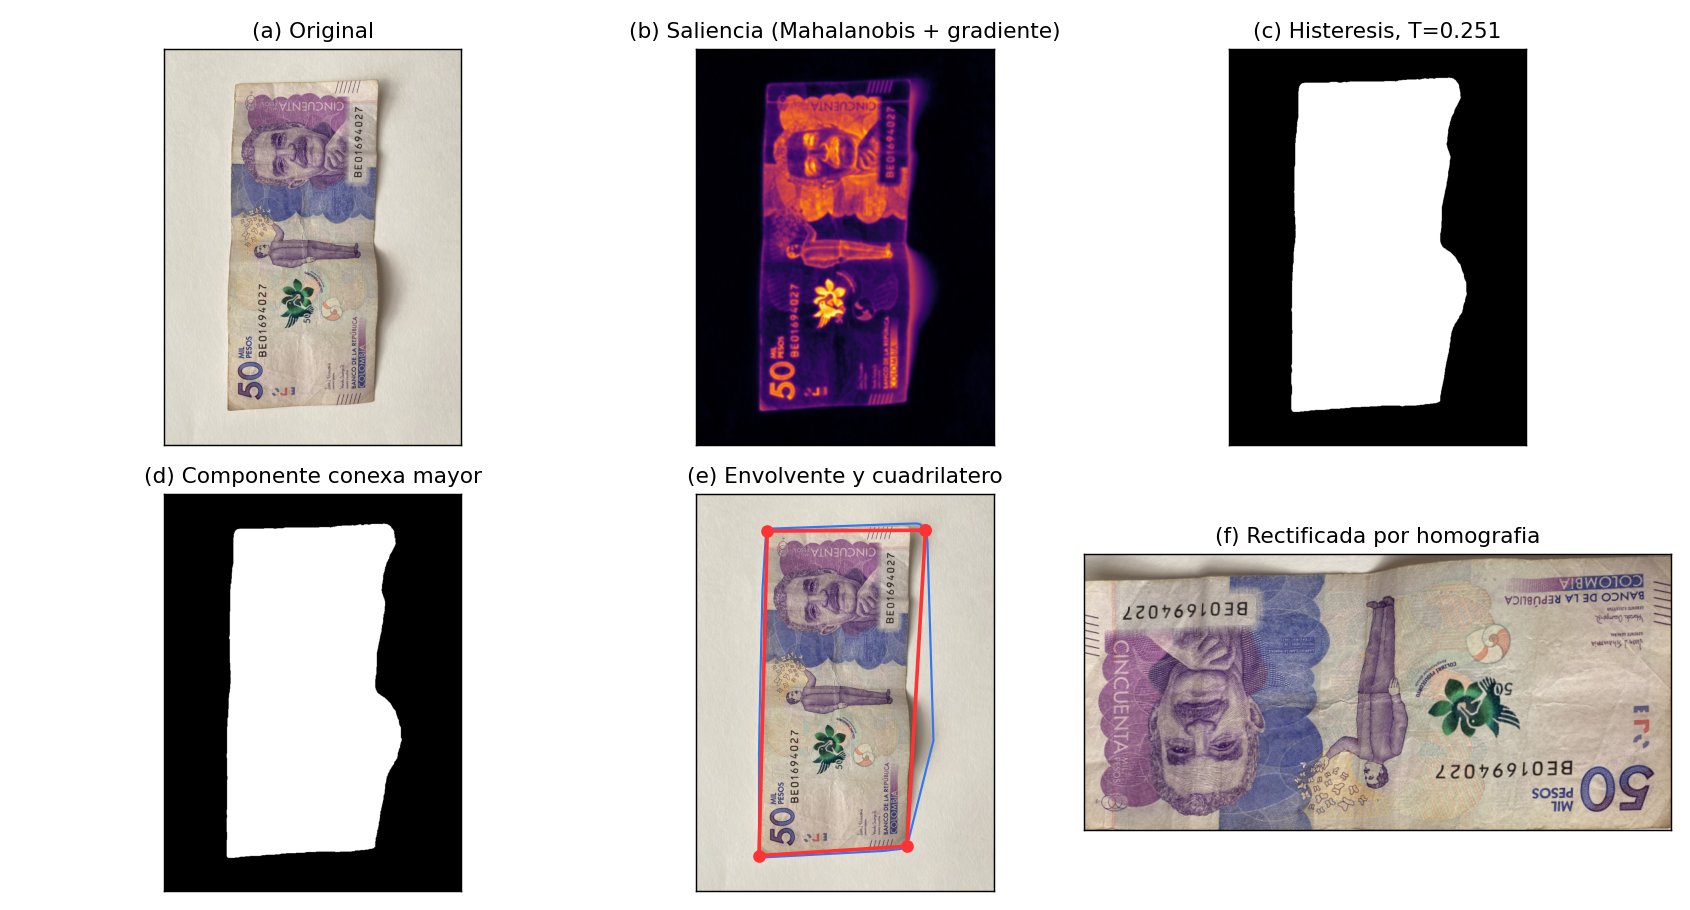
\includegraphics[width=\columnwidth]{figuras/etapas_IMG_2198.png}
\caption{Etapas del procesamiento. (a) Captura original.
(b) Mapa de saliencia. (c) Umbralización con reconstrucción geodésica.
(d) Componente conexa seleccionada. (e) Envolvente convexa en azul y
cuadrilátero de área máxima en rojo. (f) Imagen rectificada al marco
canónico.}
\label{fig:etapas}
\end{figure}

El caso que motivó la arquitectura de mapas múltiples fue el billete de
\$100.000, verde pálido sobre fondo claro: una segmentación basada en
saturación recuperaba únicamente el retrato. Los didácticos, fotografiados
sobre un tapete oscuro texturizado, produjeron el problema opuesto: la
franja perimetral mezclaba zonas muy oscuras con reflejos, la covarianza
estimada se disparaba y ningún píxel resultaba anómalo. El mapa de brillo
resuelve el segundo caso y el cromático el primero; la selección por forma
decide cuál usar en cada imagen sin intervención.

\subsection{Decisión por reglas explícitas}

El sistema no emplea ningún clasificador entrenado. No existe etapa de
aprendizaje, archivo de modelo ni parámetro ajustado por un algoritmo
de optimización. Las dos decisiones ---denominación y autenticidad---
se toman con reglas cuyas constantes están escritas en el código y
documentadas aquí.

La razón es metodológica. Un clasificador estimado sobre un conjunto
reducido tiene más parámetros libres que muestras disponibles, de modo
que su desempeño aparente no es verificable. Una regla explícita es
auditable: ante cualquier decisión puede señalarse la magnitud medida y
la constante con que se comparó. Las constantes empleadas, además, no
son arbitrarias sino que corresponden a propiedades físicas del objeto:
el color dominante de cada denominación y la energía de microtextura
que aporta la impresión calcográfica.

\subsubsection{Constancia de color}
El matiz medido de un mismo billete se desplaza decenas de grados al
cambiar la temperatura de color de la iluminación, de modo que ninguna
constante fija sería válida sin corregirlo antes. Se aplica la
hipótesis de Minkowski: para cada canal se estima el iluminante
mediante la norma $p$
\begin{equation}
e_c = \left(\frac{1}{|\Omega|}\sum_{x\in\Omega} f_c(x)^p\right)^{1/p}
\end{equation}
y se corrige dividiendo por $e_c$. Con $p=1$ se recupera la hipótesis
del mundo gris y con $p\to\infty$ la del parche blanco; se emplea
$p=6$. El iluminante se estima \emph{únicamente sobre los píxeles del
billete}: si se estimara sobre toda la imagen, el color de la mesa
entraría en el cálculo y la corrección dependería de dónde se apoyó el
billete.

El efecto es decisivo. Sin corrección, el matiz dominante del billete
de \$50.000 auténtico mide 13{,}8\textdegree\ y el del didáctico
275{,}0\textdegree, pese a ser el mismo diseño. Con corrección miden
268{,}8\textdegree\ y 275{,}8\textdegree.

\subsubsection{Regla 1: denominación por matiz dominante}
El matiz es una magnitud angular, de modo que su promedio aritmético
carece de sentido: la media de 350\textdegree\ y 10\textdegree\ no es
180\textdegree\ sino 0\textdegree. Se emplea la media circular,
\begin{equation}
\bar{H} = \arg\left(\frac{1}{n}\sum_k e^{\,j H_k}\right)
\end{equation}
acumulando solo píxeles con saturación y valor suficientes, porque el
matiz queda indefinido cuando $S\to0$ y es ruidoso cuando $V\to0$. El
módulo del vector resultante, $|\frac{1}{n}\sum_k e^{jH_k}|$, mide la
concentración: vale 1 si todos los píxeles comparten el matiz y 0 si
están uniformemente repartidos por el círculo.

La decisión es por mínima distancia angular a prototipos fijos,
\begin{equation}
d(a,b) = \min\left(|a-b| \bmod 360,\; 360 - (|a-b| \bmod 360)\right)
\end{equation}
\begin{equation}
c^{*} = \arg\min_{c} \; d\!\left(\bar{H},\, H_c\right)
\end{equation}
con $H_{50\text{mil}} = 270\textdegree$ (violeta) y
$H_{100\text{mil}} = 160\textdegree$ (verde azulado). Se rechaza la
decisión si la distancia al mejor prototipo supera una tolerancia de
55\textdegree, o si el segundo candidato queda a menos de
15\textdegree\ del primero, caso en que la decisión no sería confiable.

\subsubsection{Regla 2: autenticidad por microtextura}
\begin{equation}
V_L < \tau \;\Longrightarrow\; \text{posible reproducción impresa}
\end{equation}
donde $V_L$ es la varianza del laplaciano medida sobre el soporte del
billete en el marco canónico y $\tau = 1{,}48\times10^{-3}$.

El origen del umbral es explícito. Sobre el conjunto disponible las dos
poblaciones no se solapan: el ejemplar auténtico de menor microtextura
mide $3{,}34\times10^{-3}$ y la reproducción de mayor microtextura
$6{,}6\times10^{-4}$. El umbral se sitúa en la media geométrica de
ambos extremos,
\begin{equation}
\tau = \sqrt{3{,}34\times10^{-3} \cdot 6{,}6\times10^{-4}}
     = 1{,}48\times10^{-3}
\end{equation}
que es el punto que maximiza el margen relativo a ambos lados cuando la
magnitud se distribuye de forma multiplicativa. El margen resultante es
de un factor 2{,}3 hacia cada lado.

Que la medida se tome sobre el marco canónico es esencial: todos los
billetes se comparan al mismo tamaño en píxeles, de modo que $\tau$ es
independiente de la distancia de captura.

Se reporta además la \emph{holgura} $V_L/\tau$, expresada en factores.
Un valor de 15 significa que el billete tiene quince veces más
microtextura que el umbral y uno de 0{,}4 que tiene menos de la mitad.
Informa cuán lejos quedó la medida del límite, cosa que un simple sí o
no oculta.

\subsection{Descriptores}

\subsubsection{Patrones binarios locales}
\begin{equation}
\mathrm{LBP}_{P,R}(x_c) = \sum_{p=0}^{P-1} s(g_p-g_c)2^p,\quad
s(z)=\begin{cases}1 & z\ge0\\ 0 & z<0\end{cases}
\end{equation}
con $g_p$ el vecino situado en
$(x_c+R\cos\frac{2\pi p}{P},\,y_c-R\sin\frac{2\pi p}{P})$, obtenido por
interpolación bilineal. Se emplea la variante uniforme invariante a
rotación \cite{ojala2002}: un patrón es uniforme si el número de
transiciones circulares $U$ no supera dos, y entonces
\begin{equation}
\mathrm{LBP}^{riu2}_{P,R} =
\begin{cases}\sum_p s(g_p-g_c) & U\le2\\ P+1 & \text{si no}\end{cases}
\end{equation}
La invariancia ante cambios monotónicos de la escala de grises es
determinante aquí, porque la captura se realiza con distintos teléfonos
y bajo iluminación no controlada.

\subsubsection{Matriz de co-ocurrencia}
De $P_{d,\theta}(i,j)$ se derivan las medidas de Haralick
\cite{haralick1973}:
\begin{align}
\text{Contraste} &= \sum_{i,j}(i-j)^2P(i,j)\\
\text{Homogeneidad} &= \sum_{i,j}\frac{P(i,j)}{1+|i-j|}\\
\text{Energía} &= \sum_{i,j}P(i,j)^2\\
\text{Entropía} &= -\sum_{i,j}P(i,j)\log P(i,j)
\end{align}
La energía y la homogeneidad crecen con la regularidad de la textura y
la entropía con su desorden. Una trama de semitono regular y un
guilloche continuo difieren precisamente en esas propiedades.

\subsubsection{Análisis espectral}
\begin{equation}
F(u,v) = \sum_{x=0}^{M-1}\sum_{y=0}^{N-1}
f(x,y)e^{-j2\pi\left(\frac{ux}{M}+\frac{vy}{N}\right)}
\end{equation}
Se aplica antes una ventana de Hann separable, porque la discontinuidad
en los bordes del bloque introduce energía espuria en forma de cruz a
lo largo de los ejes de frecuencia. Se mide la razón de energía en un
anillo,
\begin{equation}
E_\rho = \frac{\sum_{(u,v)\in\mathcal{A}}|F(u,v)|^2}{\sum_{(u,v)}|F(u,v)|^2}
\end{equation}
con $\mathcal{A}=\{(u,v): \rho_1\le\rho\le\rho_2\}$ y $\rho$ el radio
normalizado respecto de Nyquist.

\subsubsection{Nitidez local}
\begin{equation}
\nabla^2 I = \frac{\partial^2I}{\partial x^2}+\frac{\partial^2I}{\partial y^2},
\quad
V_L = \frac{1}{|\Omega|}\sum_{\Omega}\left(\nabla^2I-\overline{\nabla^2I}\right)^2
\end{equation}
Toda reproducción atraviesa un muestreo adicional que actúa como filtro
pasabajas, de modo que el microtexto pierde definición.

\subsection{Criterios de rechazo}
\label{sec:rechazo}

Una medición sobre una región mal detectada es peor que ninguna
medición, porque produce cifras plausibles en apariencia. Se aplican
tres criterios, cada uno asociado a un modo de error distinto.

\begin{enumerate}
\item \textbf{Contacto con el borde}, con margen proporcional al tamaño
      de la imagen. Un billete truncado por el encuadre carece de dos
      de sus cuatro esquinas, de modo que la homografía se estimaría
      sobre un cuadrilátero que no corresponde al objeto.
\item \textbf{Relación de aspecto} fuera de $[1{,}45,\;2{,}80]$. Señala
      un billete truncado, dos billetes fusionados en una región, o un
      objeto que no es un billete.
\item \textbf{Escalón de intensidad en el contorno}. Si la intensidad
      media dentro y fuera de la región es casi la misma, la frontera
      detectada no es un borde físico sino un límite arbitrario dentro
      de una zona homogénea. Este criterio surgió de observar valores
      de agudeza de borde de 19 y de 139 en corridas intermedias, que
      son físicamente imposibles y provenían de dividir por un salto
      casi nulo.
\end{enumerate}

\subsection{Prototipo e interfaz}

El prototipo es una aplicación de escritorio que captura con la cámara
del computador y comunica el resultado por pantalla y por voz.

\subsubsection{Alcance de la dependencia externa}
Leer fotogramas de una cámara exige hablar con el controlador del
sistema operativo ---DirectShow en Windows, V4L2 en Linux,
AVFoundation en macOS--- y eso no puede escribirse en Python puro. El
proyecto aísla esa dependencia en un único módulo, del que se emplean
tres operaciones: abrir el dispositivo, leer un fotograma y cerrarlo.
De ese arreglo numérico en adelante no interviene ninguna librería
externa. No se usan funciones de extracción de contornos, de
transformación de perspectiva, de umbralización, de morfología ni de
conversión de color: todas están implementadas según se describe en
esta sección. El sistema funciona además sin cámara, analizando
fotografías ya tomadas.

\subsubsection{Verificación previa al veredicto}
Tras la rectificación se evalúan el factor de cobertura
$\kappa = A_{\text{billete}}/A_{\text{cuadro}}$, la rectangularidad y
la relación de aspecto medida. Esta última es la más informativa: la
homografía supone que el objeto es plano, de modo que un billete
plegado o visto muy oblicuamente produce un cuadrilátero cuya relación
se aparta de la nominal. Cuando algún indicador queda fuera de rango el
sistema emite una instrucción de corrección en lugar de un veredicto.
Es la conducta segura: es preferible pedir otra captura a dictaminar
sobre una imagen que la cadena no puede rectificar bien.

\subsubsection{Accesibilidad}
La interfaz enuncia la guía de colocación al abrirse, sin esperar a que
la captura falle, porque un usuario que no ve necesita saber cómo
disponer el billete antes de accionar la cámara. Dispone además de un
control para repetir el último resultado en voz y de atajos de teclado.
La síntesis se delega al motor del sistema operativo, de modo que el
prototipo hereda la voz que el usuario ya tiene configurada; si no hay
ningún motor disponible el sistema continúa en silencio sin fallar,
porque la voz complementa la salida en pantalla y no es un requisito de
funcionamiento.

\subsubsection{Criterio de redacción de la salida}
El sistema no declara en ningún caso que un billete es auténtico. Emite
``no se detectaron anomalías de impresión'' o ``posible reproducción
impresa, verifique manualmente'', y siempre remite al procedimiento
oficial del Banco de la República. Un falso negativo comunicado como
certeza podría inducir al usuario a aceptar una pérdida que de otro
modo habría evitado.

%=====================================================================
\section{Resultados Parciales}
\label{sec:resultados}

\subsection{Segmentación y rectificación}

La Fig.~\ref{fig:etapas} muestra las etapas sobre un ejemplar
auténtico. Sobre las 42 imágenes procesadas, la segmentación y
rectificación fueron válidas en \textbf{38 casos, el 90{,}5\,\%}. El
error de reproyección fue nulo hasta la precisión de máquina, como
corresponde a un sistema determinado de cuatro correspondencias.

\begin{figure}[t]
\centering
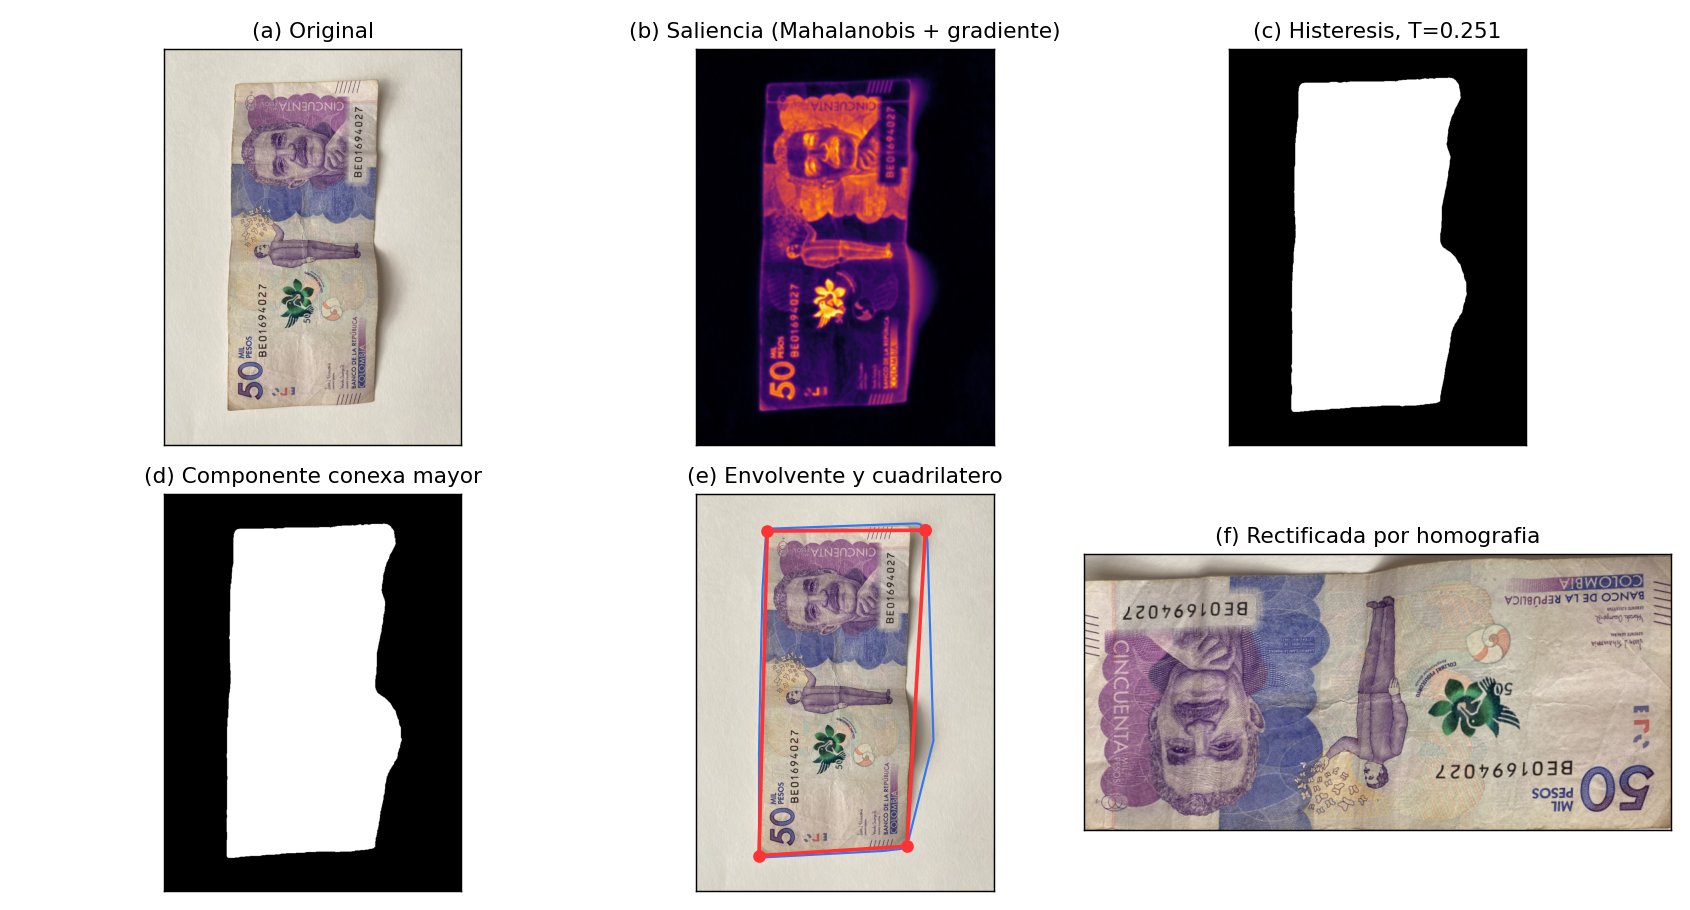
\includegraphics[width=\columnwidth]{figuras/etapas_IMG_2198.png}
\caption{Etapas del procesamiento. (a) Captura original.
(b) Mapa de saliencia. (c) Umbralización con reconstrucción geodésica.
(d) Componente conexa seleccionada. (e) Envolvente convexa en azul y
cuadrilátero de área máxima en rojo. (f) Imagen rectificada al marco
canónico.}
\label{fig:etapas}
\end{figure}

El caso que motivó la arquitectura de mapas múltiples fue el billete de
\$100.000, verde pálido sobre fondo claro: una segmentación basada en
saturación recuperaba únicamente el retrato. Los didácticos, fotografiados
sobre un tapete oscuro texturizado, produjeron el problema opuesto: la
franja perimetral mezclaba zonas muy oscuras con reflejos, la covarianza
estimada se disparaba y ningún píxel resultaba anómalo. El mapa de brillo
resuelve el segundo caso y el cromático el primero; la selección por forma
decide cuál usar en cada imagen sin intervención.

\subsection{Reconocimiento de denominación}

Sobre los 34 ejemplares con segmentación válida de las dos
denominaciones modeladas, la Regla 1 acertó en el \textbf{100\,\%} de
los casos, sin rechazos (12 de \$100.000 y 22 de \$50.000). Como no hay
entrenamiento, no hace falta partición ni validación cruzada: las
constantes son fijas y la evaluación consiste en aplicarlas.

La cifra debe leerse con cautela por una razón concreta. Se evaluó
también el comportamiento ante seis imágenes de denominaciones no
modeladas, y solo tres fueron rechazadas correctamente. El billete de
\$5.000 mide 262{,}7\textdegree\ de matiz dominante, apenas
7\textdegree\ del prototipo de \$50.000, y el de \$2.000 queda a
50\textdegree. \textbf{El matiz por sí solo no separa las
denominaciones violetas entre sí.} Distinguirlas exigiría incorporar el
tamaño físico o características estructurales, y hasta entonces el
alcance del reconocimiento se limita a las dos denominaciones
declaradas.

\subsection{Autenticidad por regla de umbral}

Sobre las 40 imágenes con segmentación válida, la Regla 2 clasificó
correctamente las 40: treinta auténticas y diez reproducciones, sin
falsos positivos ni falsos negativos. Las poblaciones no se solapan:

\begin{center}
\small
\begin{tabular}{@{}lcc@{}}
\toprule
 & \textbf{mínimo} & \textbf{máximo} \\
\midrule
Auténticos ($n=30$)     & $3{,}34\times10^{-3}$ & $2{,}65\times10^{-2}$ \\
Reproducciones ($n=10$) & $1{,}7\times10^{-4}$  & $6{,}6\times10^{-4}$ \\
\midrule
Umbral $\tau$           & \multicolumn{2}{c}{$1{,}48\times10^{-3}$} \\
\bottomrule
\end{tabular}
\end{center}

El auténtico de menor microtextura tiene 5{,}1 veces más energía en el
laplaciano que la reproducción de mayor microtextura. Ese margen, y no
la exactitud del 100\,\%, es el indicador informativo: una exactitud
perfecta sobre 40 muestras es compatible con muchas configuraciones,
mientras que un margen de factor 5 indica cuánto tendría que cambiar la
calidad de impresión de una reproducción para engañar al sistema.

\subsection{Comparación elemental y diagramas de caja}

Antes de fijar cualquier regla se verificó si las clases se separan con
estadísticos de primer y segundo orden, calculados sobre el billete ya
segmentado y sin fondo. La Fig.~\ref{fig:cajas} presenta los
diagramas de caja y bigotes, con los puntos individuales superpuestos
porque las muestras son pequeñas.

\begin{figure}[t]
\centering
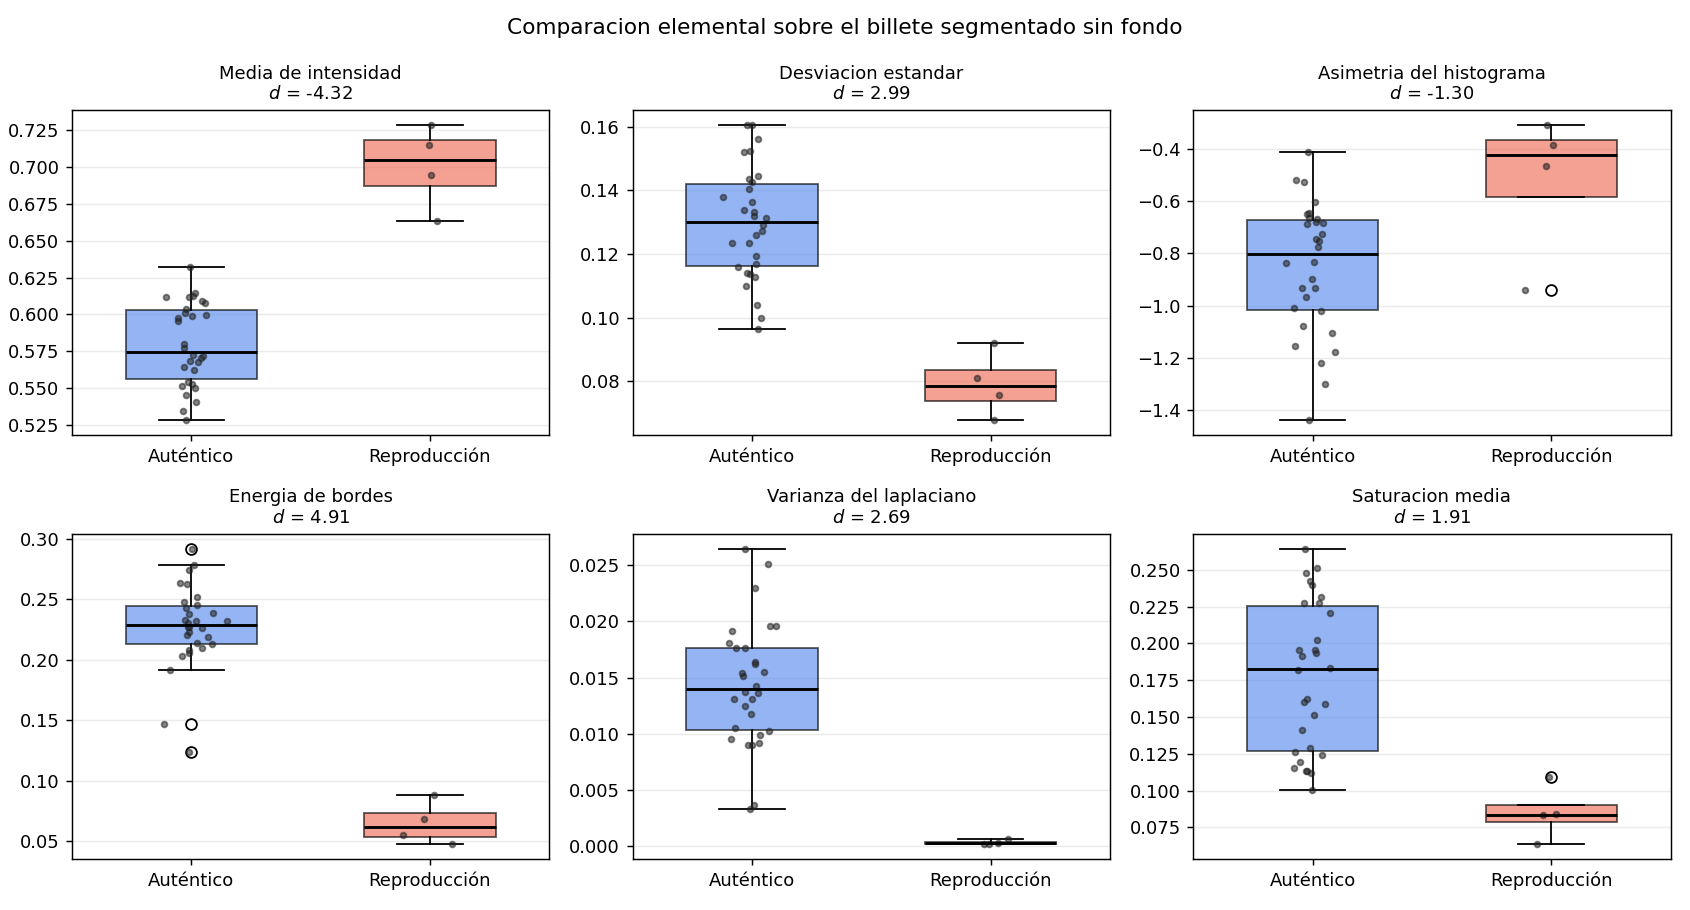
\includegraphics[width=\columnwidth]{figuras/cajas_bigotes.png}
\caption{Comparación elemental entre clases sobre el billete segmentado
sin fondo. Se indica el tamaño del efecto de Cohen.}
\label{fig:cajas}
\end{figure}

El resultado más informativo es negativo: \textbf{la media de intensidad
no separa las clases} en el conjunto inicial ($d = 0{,}54$, cajas
solapadas). Lo que separa es la energía de bordes y la varianza del
laplaciano. El tamaño del efecto de Cohen,
\begin{equation}
d = \frac{\mu_1-\mu_2}{s_p},\quad
s_p = \sqrt{\frac{(n_1-1)s_1^2+(n_2-1)s_2^2}{n_1+n_2-2}}
\end{equation}
se prefiere a una prueba de significancia porque no depende del tamaño
muestral, lo que importa con muestras reducidas.

\subsection{Mapas de saliencia sobre el billete segmentado}

La Fig.~\ref{fig:saliencia} contrasta un ejemplar auténtico de
\$50.000 con una reproducción de la misma denominación. Ambas filas
comparten escala de color: si cada mapa se normalizara por separado,
los dos ocuparían todo el rango y un billete sin microtextura se vería
tan brillante como uno que sí la tiene.

\begin{figure*}[t]
\centering
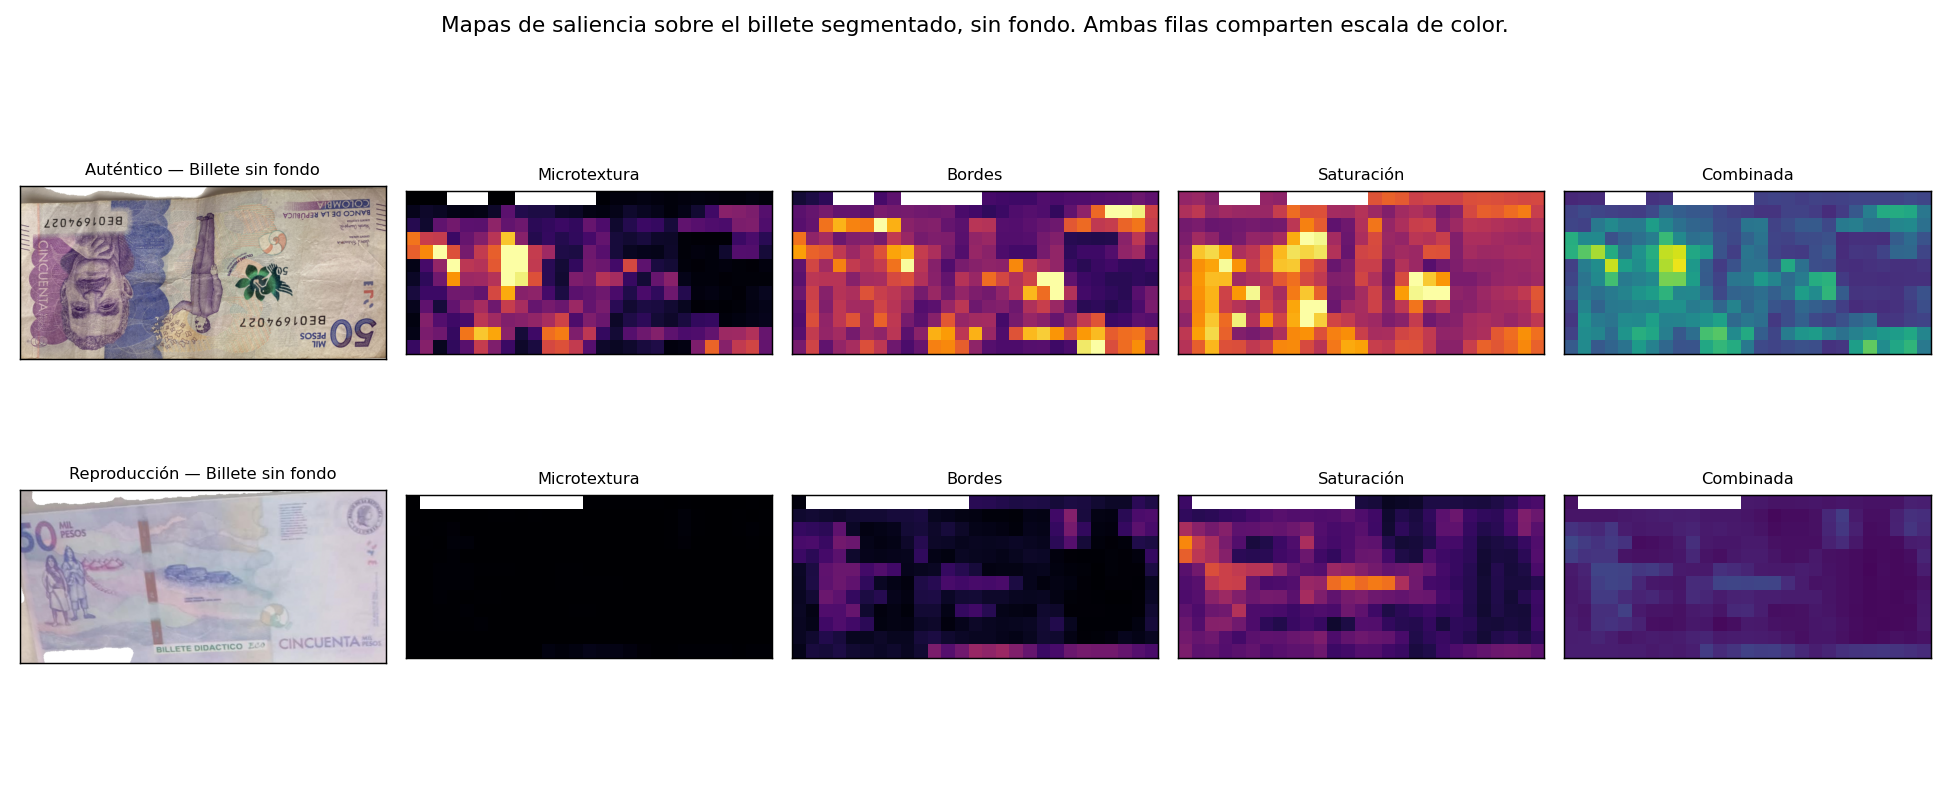
\includegraphics[width=\textwidth]{figuras/saliencia_billete_IMG_2198.png}
\caption{Mapas de saliencia calculados sobre el billete ya segmentado
y sin fondo. Arriba un ejemplar auténtico, abajo una reproducción de
la misma denominación. Ambas filas comparten escala de color. El mapa
de microtextura de la reproducción es prácticamente nulo en toda su
extensión.}
\label{fig:saliencia}
\end{figure*}

\begin{table}[h]
\centering
\caption{Promedios sobre el soporte del billete}
\label{tab:saliencia}
\small
\begin{tabular}{@{}lccc@{}}
\toprule
 & \textbf{Auténtico} & \textbf{Reproducción} & \textbf{Cociente} \\
\midrule
Microtextura & 0{,}02456 & 0{,}00031 & 0{,}013 \\
Bordes       & 0{,}2862  & 0{,}0706  & 0{,}247 \\
Saturación   & 0{,}1936  & 0{,}0862  & 0{,}445 \\
\bottomrule
\end{tabular}
\end{table}

El resultado más informativo es la distribución espacial. En el
ejemplar auténtico la microtextura se concentra sobre las zonas de
guilloche y de microtexto, con celdas muy brillantes y otras oscuras;
en la reproducción el mapa es uniformemente nulo, lo que indica que la
pérdida no afecta a una región concreta sino a toda la superficie
impresa. Eso es coherente con el mecanismo físico propuesto: no se
trata de que la copia reproduzca mal algún elemento, sino de que la
cadena de impresión de consumo no reproduce microestructura en
absoluto.

La saturación es la evidencia menos discriminante de las tres, con un
cociente de $0{,}445$ frente al $0{,}013$ de la microtextura. Por eso
recibe el menor peso en la combinación.

\subsection{El problema de la confusión con la captura}
\label{sec:pareado}

Las medidas que más separaban ---energía de bordes y nitidez--- son
precisamente las que degrada una fotografía tomada en condiciones
distintas. Con las dos clases capturadas en sesiones, fondos y
dispositivos diferentes, no era posible atribuir la separación a la
impresión. Se realizaron dos pruebas de descarte.

\subsubsection{Compresión}
Se degradaron las imágenes auténticas con la misma cadena de reescalado
y compresión JPEG de las reproducciones. La varianza del laplaciano se
mantuvo entre 0{,}012 y 0{,}017 frente a 0{,}0003 de las
reproducciones. \textbf{La compresión no explica la diferencia.}

\subsubsection{Enfoque}
Se definió la agudeza del borde físico del papel,
\begin{equation}
\text{agudeza} = \frac{\langle|\nabla I|\rangle_{\text{banda}}}
{\left|\bar{I}_{\text{dentro}} - \bar{I}_{\text{fuera}}\right|}
\end{equation}
que es el inverso de la anchura de transición, en $1/\text{píxel}$. Ese
borde es un escalón real de la escena, idéntico en un billete auténtico
y en uno didáctico, y su anchura depende únicamente del enfoque y del
movimiento de la cámara, no de cómo esté impreso el billete. Las
reproducciones dieron $1{,}87 \pm 1{,}66$ frente a
$0{,}87 \pm 0{,}27$ de los auténticos, es decir estaban igual o mejor
enfocadas. \textbf{El desenfoque tampoco explica la diferencia.}

\subsection{Experimento pareado}

Ninguna prueba de descarte agota las alternativas. Se adoptó entonces un
diseño que controla la condición de captura por construcción en lugar de
por argumentación: \textbf{fotografiar un billete auténtico y uno
didáctico de la misma denominación dentro del mismo encuadre}. Ambos
comparten sensor, exposición, balance de blancos, distancia focal,
instante e iluminación. Es el equivalente fotográfico de un experimento
pareado: se compara dentro de cada unidad experimental en lugar de entre
grupos independientes, lo que elimina la varianza entre unidades.

La identificación de cada ejemplar es verificable y no supuesta: las
reproducciones de curso legal deben diferir en tamaño, y dentro de un
mismo encuadre la escala es común, de modo que el área en píxeles es
directamente comparable.

\begin{table}[h]
\centering
\caption{Comparación pareada. Didáctico como cociente del auténtico}
\label{tab:pareado}
\small
\begin{tabular}{@{}lccc@{}}
\toprule
\textbf{Medida} & \textbf{\$50.000} & \textbf{\$100.000} & \textbf{Prom.} \\
\midrule
Media de intensidad        & 1{,}31 & 1{,}18 & 1{,}24 \\
Desviación estándar        & 0{,}78 & 0{,}53 & 0{,}65 \\
Energía de bordes          & \textbf{0{,}34} & \textbf{0{,}26} & \textbf{0{,}31} \\
Varianza del laplaciano    & \textbf{0{,}04} & \textbf{0{,}01} & \textbf{0{,}04} \\
Saturación media           & 0{,}71 & 0{,}80 & 0{,}76 \\
Agudeza del borde físico   & 2{,}70 & 1{,}37 & 2{,}14 \\
\midrule
Lado mayor (tamaño)        & 0{,}860 & 0{,}746 & --- \\
\bottomrule
\end{tabular}
\end{table}

\begin{figure}[t]
\centering
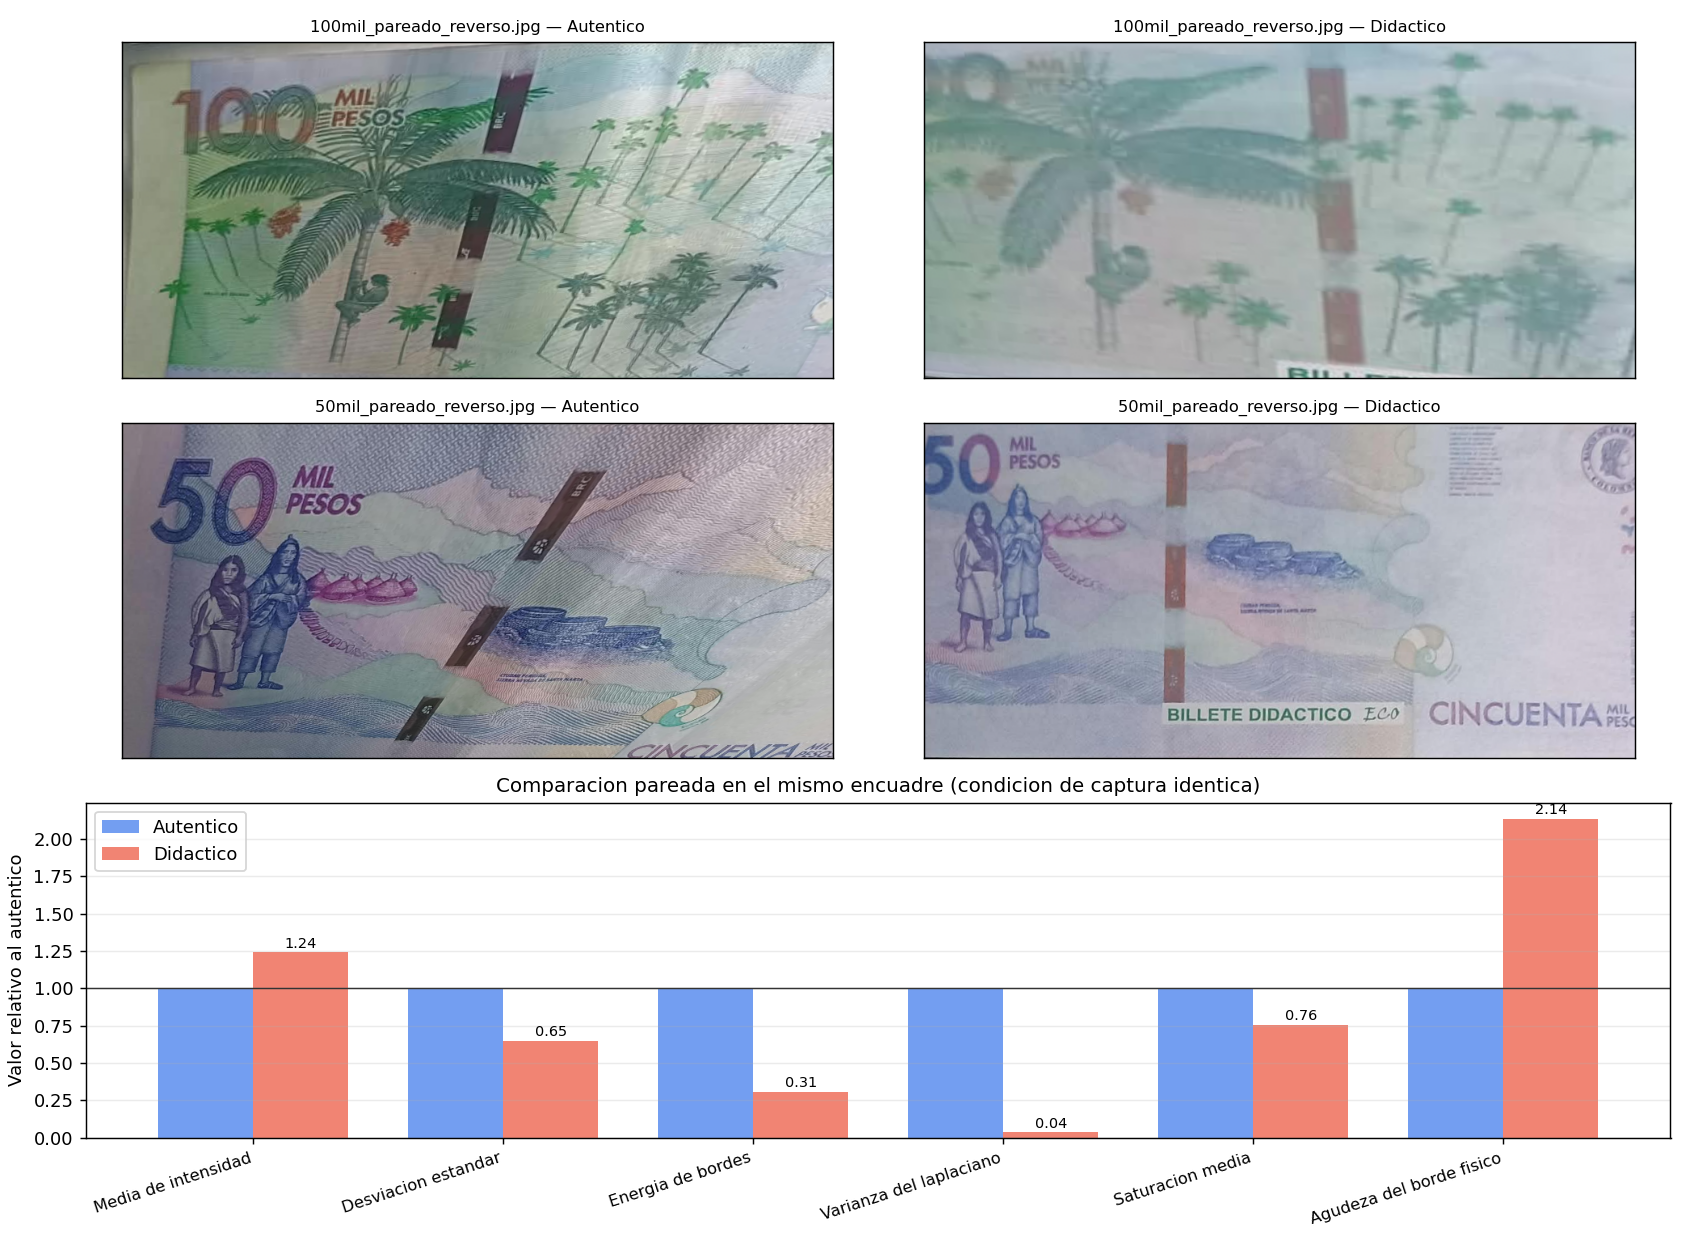
\includegraphics[width=\columnwidth]{figuras/comparacion_pareada.png}
\caption{Comparación pareada en el mismo encuadre. Arriba, los billetes
rectificados de cada par. Abajo, las medidas del didáctico relativas al
auténtico.}
\label{fig:pareado}
\end{figure}

\textbf{Conclusión.} Las reproducciones presentan entre 25 y 100 veces
menos energía en el laplaciano, y lo hacen mientras su borde físico está
\emph{más} enfocado (2{,}14 veces en promedio). La pérdida de
microtextura no puede atribuirse al desenfoque. Las dos denominaciones
coinciden en dirección y en orden de magnitud, lo que descarta que se
trate de una peculiaridad de un ejemplar. La diferencia de
microestructura entre la impresión de seguridad y la reproducción es
medible con una cámara convencional en luz reflejada.

De las cuatro fotografías pareadas, dos fueron descartadas por los
criterios de la Sección~\ref{sec:rechazo} sin intervención manual: en
los anversos de ambas denominaciones alguno de los billetes quedó
cortado por el borde del cuadro.

\subsection{Prototipo}

El prototipo se probó de extremo a extremo. Ante un ejemplar auténtico
de \$50.000 devolvió la denominación correcta, una holgura de 15{,}5
veces el umbral y el mensaje ``no se detectaron anomalías de
impresión''; ante el didáctico de \$100.000, una holgura de 0{,}11 y la
advertencia correspondiente. Ante una fotografía tomada oblicuamente,
con relación de aspecto medida de 3{,}04, no emitió veredicto sino la
indicación de que la fotografía no es utilizable.

Como no hay modelo que cargar ni etapa de entrenamiento, la aplicación
se ejecuta directamente. El tiempo de procesamiento es de
aproximadamente un segundo por imagen reducida a 1024 píxeles de lado
mayor. Ante una fotografía tomada oblicuamente
---relación de aspecto medida de 3{,}04--- no emitió veredicto sino la
instrucción de colocar el billete plano y de frente. El tiempo de
procesamiento es de aproximadamente un segundo por imagen reducida a
1024 píxeles de lado mayor.

\subsection{Hallazgo sobre el tamaño}

Las reproducciones midieron entre 14\,\% y 25\,\% menos que el billete
que representan, diferencia exigida por la normativa. Es el
discriminador más simple concebible y \textbf{el sistema no puede
utilizarlo}, porque la rectificación al marco canónico normaliza el
tamaño por construcción. Aprovecharlo exigiría una referencia de escala
en la escena. Se reporta como limitación consciente del diseño.

\subsection{Reproducibilidad}

Todas las cifras son reproducibles ejecutando en orden
\texttt{src/evaluar.py}, \texttt{scripts/comparacion\_simple.py} y
\texttt{scripts/comparacion\_pareada.py} sobre el conjunto que acompaña
la entrega. El tiempo total es de unos cinco minutos en un computador
portátil sin aceleración por hardware.

\subsection{Limitaciones de estos resultados}

\begin{enumerate}
\item El conjunto pareado consta de dos pares válidos. Confirma la
      existencia del fenómeno, no su magnitud poblacional.
\item Las reproducciones son billetes didácticos comerciales. No
      representan falsificaciones producidas con intención de engañar,
      que emplean mejores sustratos y técnicas.
\item Solo se evaluaron dos denominaciones en el reconocimiento, de
      colores muy distintos.
\item La verificación de encuadre es posterior a la captura, no una
      guía continua en tiempo real.
\item No se ha evaluado la generalización entre dispositivos.
\item El reconocimiento por matiz no separa las denominaciones de
      color violeta entre sí, como muestra el caso de \$5.000.
\end{enumerate}

%=====================================================================
\section{Trabajo Siguiente}

Ampliar el conjunto pareado a las denominaciones restantes y a los
anversos, dejando ambos billetes completos y separados dentro del
cuadro. Incorporar la verificación de la tinta ópticamente variable del
billete de \$100.000 mediante el desplazamiento de matiz entre dos
capturas a ángulos distintos. Ejecutar el protocolo de variación
sistemática de dispositivo, iluminación y fondo para medir la
generalización. Validar la interfaz con usuarios.

La continuación natural del prototipo es su traslado a un dispositivo
móvil con captura en vivo. Esa es la forma en que el sistema tiene
utilidad real, porque la verificación debe ocurrir en el lugar de la
transacción y no frente a un computador. El traslado no exige
rediseñar el algoritmo, que opera sobre cualquier fotografía con
independencia de su origen, pero sí añade dos problemas propios que
esta etapa no aborda: la guía de encuadre en tiempo real para un
usuario que no ve la pantalla, y la ejecución de la cadena a una tasa
suficiente para dar realimentación continua.

\section{Consideraciones Éticas y Legales}

La reproducción de billetes de curso legal está regulada en Colombia y
la falsificación de moneda constituye un delito. Las reproducciones
generadas en laboratorio se producirán exclusivamente con fines
académicos, bajo supervisión del docente, se marcarán de forma indeleble
como muestra de investigación, no se pondrán en circulación bajo ninguna
circunstancia y se destruirán al finalizar el proyecto. El sistema no
emite en ningún caso un veredicto de autenticidad positiva, y toda
salida remite al procedimiento oficial de verificación del Banco de la
República.

%=====================================================================
\begin{thebibliography}{9}

\bibitem{berenguel2016}
A. Berenguel, O. Ramos Terrades, J. Lladós y C. Cañero,
``Banknote counterfeit detection through background texture printing
analysis,'' en \textit{Proc. 12th IAPR Int. Workshop on Document
Analysis Systems (DAS)}, Santorini, Grecia, 2016, pp. 66--71.
doi: 10.1109/DAS.2016.44.

\bibitem{dewaele2016}
T. Dewaele, M. Diephuis, T. Holotyak y S. Voloshynovskiy,
``Forensic authentication of banknotes on mobile phones,'' en
\textit{Proc. IS\&T Int. Symp. on Electronic Imaging: Media
Watermarking, Security, and Forensics}, San Francisco, EE.UU., 2016,
pp. 1--8. doi: 10.2352/ISSN.2470-1173.2016.8.MWSF-083.

\bibitem{ecounterfeit2017}
A. Berenguel, O. Ramos Terrades, J. Lladós y C. Cañero,
``e-Counterfeit: A mobile-server platform for document counterfeit
detection,'' en \textit{Proc. 14th IAPR Int. Conf. on Document Analysis
and Recognition (ICDAR)}, Kioto, Japón, 2017, pp. 15--20.
doi: 10.1109/ICDAR.2017.390.

\bibitem{huaytalla2021}
B. Huaytalla, D. Humari y G. Kemper,
``An algorithm for Peruvian counterfeit banknote detection based on
digital image processing and SVM,''
\textit{Advances in Science, Technology and Engineering Systems
Journal}, vol. 6, no. 1, pp. 1171--1178, 2021.
doi: 10.25046/aj0601132.

\bibitem{salem2022}
T. K. Salem, W. K. Wong, T. S. Min y E. K. Wong,
``One- and Five-Ringgit Malaysia banknotes reader with counterfeit
detection for visually impaired person using backlight mechanism and
image processing techniques,''
\textit{F1000Research}, vol. 10, art. 1098, 2022.
doi: 10.12688/f1000research.58446.2.

\bibitem{berenguel2019}
A. Berenguel Centeno, O. Ramos Terrades, J. Lladós Canet y
C. Cañero Morales,
``Identity document and banknote security forensics: A survey,''
\textit{arXiv preprint} arXiv:1910.08993, 2019.

\bibitem{ojala2002}
T. Ojala, M. Pietikäinen y T. Mäenpää,
``Multiresolution gray-scale and rotation invariant texture
classification with local binary patterns,''
\textit{IEEE Transactions on Pattern Analysis and Machine
Intelligence}, vol. 24, no. 7, pp. 971--987, 2002.
doi: 10.1109/TPAMI.2002.1017623.

\bibitem{haralick1973}
R. M. Haralick, K. Shanmugam e I. Dinstein,
``Textural features for image classification,''
\textit{IEEE Transactions on Systems, Man, and Cybernetics},
vol. SMC-3, no. 6, pp. 610--621, 1973.
doi: 10.1109/TSMC.1973.4309314.

\bibitem{otsu1979}
N. Otsu,
``A threshold selection method from gray-level histograms,''
\textit{IEEE Transactions on Systems, Man, and Cybernetics}, vol. 9,
no. 1, pp. 62--66, 1979. doi: 10.1109/TSMC.1979.4310076.

\bibitem{rosenfeld1966}
A. Rosenfeld y J. L. Pfaltz,
``Sequential operations in digital picture processing,''
\textit{Journal of the ACM}, vol. 13, no. 4, pp. 471--494, 1966.
doi: 10.1145/321356.321357.

\bibitem{andrew1979}
A. M. Andrew,
``Another efficient algorithm for convex hulls in two dimensions,''
\textit{Information Processing Letters}, vol. 9, no. 5, pp. 216--219,
1979. doi: 10.1016/0020-0190(79)90072-3.

\bibitem{banrep}
Banco de la República de Colombia,
``Nueva familia de billetes: preguntas frecuentes.'' [En línea].
Disponible: \url{https://www.banrep.gov.co/es/nueva-familia-billetes-preguntas}
[Consultado: septiembre de 2026].

\end{thebibliography}

\end{document}
